%%%%%%%%%%%%%%%%%%%%%%%%%%%%%%%%%%%%%%%%%%%%%%%%%%%%%%%%%%%%%%%%%%%%%%%%%%%%%%%%%%%%%%%%%%%%%%%
%%%%%%%%%%%%%%%%%%%%%%%%%%%%%%%%%%%%%%%%%%%%%%%%%%%%%%%%%%%%%%%%%%%%%%%%%%%%%%%%%%%%%%%%%%%%%%%
%% LaTeX-Beamer template for KIT design
%% by Erik Burger, Christian Hammer
%% title picture by Klaus Krogmann
%%
%% version 2.1
%%
%% mostly compatible to KIT corporate design v2.0
%% http://intranet.kit.edu/gestaltungsrichtlinien.php
%%
%% Problems, bugs and comments to
%% burger@kit.edu
%%
%%
%% Modified: 30.1.2013, Schwall

\documentclass[12pt]{beamer}

%% SLIDE FORMAT
\usepackage{templates/beamerthemekit}

%% german time format (e.g 30.1.2013)
\usepackage{datetime}
\usepackage{bbm} %% Used to denote the indicator function
%\usepackage[T1]{fontenc}
\usepackage{amsmath}
\usepackage{amssymb}
\usepackage{amsfonts}
\usepackage{amsthm}
\usepackage{graphicx}
\usepackage{subfig}

\newdateformat{germandate}{\THEDAY.\THEMONTH.\THEYEAR}
\newdateformat{americandate}{\THEMONTH/\THEDAY/\THEYEAR}

% use these packages for PCM symbols and UML classes
\usepackage{templates/tikzkit}
\usepackage{templates/tikzuml}
\usepackage{siunitx}

\usepackage{times}
\usepackage{tikz}


\usepackage[english]{babel}
\usepackage{csquotes}
\setquotestyle{american}
\usepackage[language=american,autocite=footnote,citestyle=authortitle,citetracker=true,backend=biber,babel=other]{biblatex}
\addbibresource{../refs.bib}

\usepackage{verbatim}
\usetikzlibrary{arrows,shapes}

\setbeamerfont{footnote}{size=\tiny}
%%%%%%%%%%%%%%%%%%%%%%%%%%%%%%%%%%%%%%%%%%%%%%%%%%%%%%%%%%%%%%%%%%%%%%%%%%%%%%%%%%%%%%%%%%%%%%%
%%%%%%%%%%%%%%%%%%%%%%%%%%%%%%%%%%%%%%%%%%%%%%%%%%%%%%%%%%%%%%%%%%%%%%%%%%%%%%%%%%%%%%%%%%%%%%%
% the presentation starts here

\usepackage{datetime}
\newdate{date}{03}{09}{2014}

% english vs. ngerman
\selectlanguage{english}

\title[Operating Characteristics of Underlay Cognitive Relay Networks]{Operating Characteristics of Underlay Cognitive Relay Networks}
\subtitle{Presentor: Noha El Gemayel}
\author[Ankit.Kaushik@kit.edu]{Ankit Kaushik, Ralph Tanbourgi, Friedrich K. Jondral}% \\ \textbf{Presenter: Noha El Gemayel}}

%% insert date in correct format
\iflanguage{english}{
	\date{3 September 2014}
	}{
	\date{\germandate\today}
}

\institute{Communications Engineering Lab}

% Bibliography

%\usepackage[citestyle=authoryear,bibstyle=numeric,hyperref,backend=biber]{biblatex}
%\addbibresource{templates/example.bib}
%\bibhang1em
\newcommand{\e}[2]{{\mathbb E}_{#1} {\left[ #2 \right]}}
\newcommand{\p}{\mathbb P}
\newcommand{\B}{\mathcal{B}}
\DeclareMathOperator*{\argmax}{arg\,max}
\newcommand{\eqdef}{\mathrel{\mathop:}=}
\newcommand{\fs}[1]{\fontsize{ #1 pt}{8.2}\selectfont}
\DeclareMathOperator*{\erf}{erf}
% Variable parameters
%\newcommand{\var_interf_outage_x_pos}{301}
%\newcommand{\var_interf_outage_y_pos}{216.6}
\newcommand{\sub}[1]{_{\text{#1}}}
\DeclareSIUnit{\microsecond}{\ensuremath{\mu}s}
\DeclareMathOperator*{\Pro}{Pr}
\DeclareMathOperator*{\maxi}{max}
\DeclareMathOperator*{\expec}{\mathbb{E}}
\DeclareMathOperator*{\gthan}{\ge}
\DeclareMathOperator*{\eqto}{=}
\DeclareMathOperator*{\cosi}{ci}
\DeclareMathOperator*{\sini}{si}
\newtheorem{lem}{Lemma}
\newtheorem{prop}{Proposition}
\newtheorem{remark}{Remark}
\newtheorem{coro}{Corollary}
\newtheorem{defi}{Definition}


% Position the text inside the frame
\usepackage[absolute,overlay]{textpos}

\addtobeamertemplate{footnote}{}{\vspace{1.0ex}}
\addtolength{\footnotesep}{-5mm} % change to 1mm

\begin{document}

\newcommand\FrameText[1]{%
  \begin{textblock*}{\paperwidth}(0pt,\textheight)
    \raggedright #1\hspace{.5em}
  \end{textblock*}}

\setbeamerfont{normal text}{size=\small}


%title page
\begin{frame}
	\titlepage
\end{frame}

\section{Contents}
%%%%%%%%%%%%%%%%%%%%%%%%%%%%%%%%%%%%%%%%%%%%%%%%%%%% Frame %%%%%%%%%%%%%%%%%%%%%%%%%%%%%%%%%%%%%%%%%%%%%%%%%%%%%%	
\begin{frame}{Contents}
 	%\fs{10}
	\fontsize{10 pt}{15}\selectfont
	\begin{itemize}	
		\item Problem statement 
		\item System model 
		\item Interference Analysis 
		\item Conclusion 
	\end{itemize}
\end{frame}

\section{Problem Statement}
%%%%%%%%%%%%%%%%%%%%%%%%%%%%%%%%%%%%%%%%%%%%%%%%%%%% Frame %%%%%%%%%%%%%%%%%%%%%%%%%%%%%%%%%%%%%%%%%%%%%%%%%%%%%%
\begin{frame}{Problem Statement}
		%\vspace{-0.5cm}
		\begin{overlayarea}{\textwidth}{4.4cm}
       	  	       	\begin{figure}
			\centering
        	        	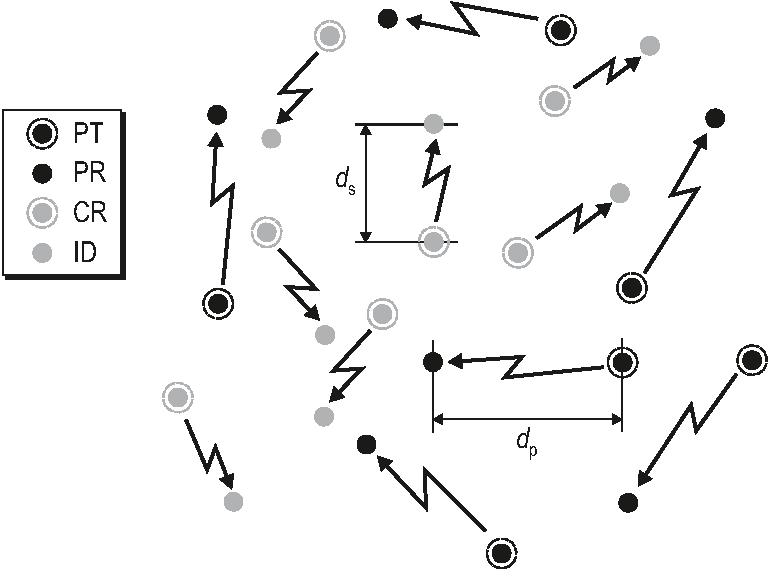
\includegraphics[trim=0.0cm 0.0cm 0.0cm 0.0cm,clip=true,width=0.4 \paperwidth]{../figures/SGeometry}
			\end{figure}
		\end{overlayarea} 
		\begin{overlayarea}{\textwidth}{2.8cm}
		\only<1>
		{
			Motivation:
			\fs{8}
			\begin{itemize}
				\item Goldsmith \textit{et. al.} described different paradigms for shared access: overlay, underlay and interweave.
				\item For the underlay system it is important to characterize the interference caused by other transmitters in the system namely, PT and ST.
				\item At network level, stochastic geometry (SG) offers an analytical tractable model to characterize interference at PRs and SRs and perform analysis for CRN.
%Notes: At the network level stochastic geometry captures the variations in the interference due to the random node locations, node mobility and fading. 
%Notes: In this way, SG provides a probabilistic model for studying interference statistics. 	
			\end{itemize}	
		}
		\only<2>
		{
			Issues:
			\fs{8}
			\begin{itemize}
				\item Systems with sensing are prone to imperfections. 
%Notes:Sensing is included in the CRN to reduce interference. However, due to sensing errors, the CRN is prone to imperfections.			
				\item Also, sensing introduces dependency in the model, ignoring this dependency may distort the true performance of the system.
				\item In most works, the performance of the CRN is restricted to the outage probability at the PRs only. 
				%Notes: Moreover, in most works, the performance of the CRN is restricted to the outage probability at the PRs only. Outage at SRs is either not considered or dealt separately for the system optimization. 	
			\end{itemize}
		}
		\only<3>
		{
			Contributions:
		       	\fs{8}
			\begin{itemize}
				 \item We do not perform sensing, we are able to obtain exact closed-form expressions. 
				 %Notes:i We do not perform sensing, we are able to obtain exact closed-form expressions for the distribution function of the signal-to-interference ratio ($\textsf{SIR}$) at PR and SR.			
				 \item The expressions obtained from our model can serve as a lower performance bound (LPB). 
				 \item We consider outage probability constraints at the PR and SR jointly and derive operating characteristics (OC) for the CRN.
 				 \item We perform the quantitative analysis for the CRN operating in indoor and outdoor scenarios. 
%Notes:Finally, we employ the OC to quantitatively analyze and compare the performance of the primary and secondary systems operating indoor, a scenario illustrated in Kaushik \textit{et. al.}, and outdoor.  
			\end{itemize}	
		}
		\end{overlayarea}
	
	\only<1>
	{
	%		\footcitetext{Goldsmith09}
	}
	\only<2>
	{
	%	\footcitetext{Tan12}	
	}
	\only<3>
	{
	%	\footcitetext{Kaushik13}
	}
\end{frame}

\section{System Model}
%%%%%%%%%%%%%%%%%%%%%%%%%%%%%%%%%%%%%%%%%%%%%%%%%%%% Frame %%%%%%%%%%%%%%%%%%%%%%%%%%%%%%%%%%%%%%%%%%%%%%%%%%%%%%	
\begin{frame}{System Model}
        \begin{columns}
        \begin{column}{0.49\paperwidth}
		\fs{8}
		\begin{itemize}	
			%Notes: CR is a network element that intends to fulfill the spectral requirements of the IDs.
			%Notes: For downlink transmission from CR to ID, CR and ID correspond to ST and SR.
			\item<1-> We assume the same transmit power for all CRs $P\sub{s}$ and preclude any form of cooperation or coordination among them.
			\item<1-> We do not involve sensing at CRs, $P\sub{s}$ can be regulated to sustain the constraint at the PR. 
			\item<2-> Network Layer: \\ {
				PTs and STs/CRs are modelled by a stationary 2-D PPP $\Phi\sub{PT}$, $\Phi\sub{CR}$ with densities $\lambda\sub{p}$, $\lambda\sub{s}$.}
			\item<3-> Medium Access layer: \\{
All active PTs and CRs follow a time synchronous slotted medium access.}
			%Notes: Applying independent thinning property of PPP, $\lambda\sub{p}$, $\lambda\sub{s}$ include $\beta$ for the PT and CR. 
			\item<4-> Physical layer: \\
{
All transmitted signals undergo distance dependent path loss $\| \cdot \|^{-\alpha}$, where $\alpha>2$ and frequency-flat Rayleigh fading.}
			%Notes: To focus our analysis to the scenario described in Kaushik \textit{et. al.}, $d\sub{p} \ge d\sub{s}$ and $\lambda\sub{p} \le \lambda\sub{s}$
			%Notes: $\alpha$ is same for the primary and secondary system.	
	\end{itemize}
	\end{column}
        \begin{column}{0.49\paperwidth}
		\fs{8}
		%\begin{overlayarea}{\textwidth}{4.4cm}
       	  	\begin{figure}
			\centering
        		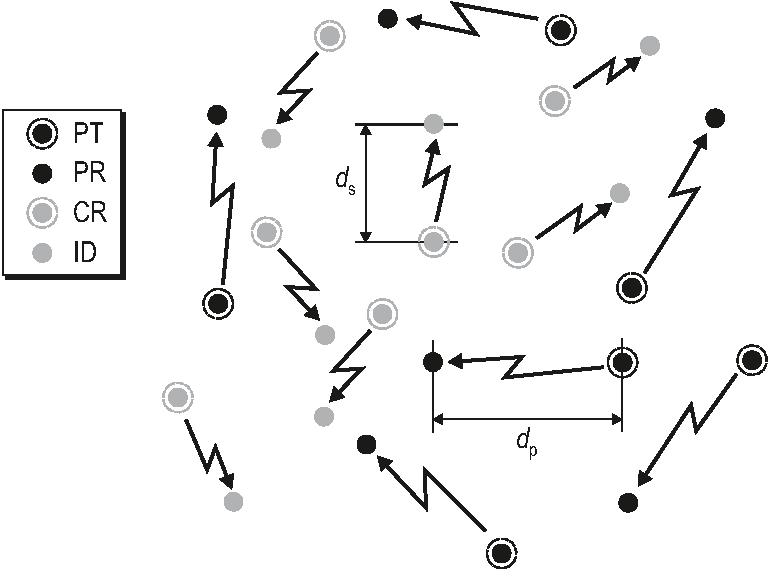
\includegraphics[trim=0.0cm 0.0cm 0.0cm 0.0cm,clip=true,width=0.4 \paperwidth]{../figures/SGeometry}
			\end{figure}
	\end{column}
	\end{columns}
\end{frame}

\section{Interference Analysis}
%%%%%%%%%%%%%%%%%%%%%%%%%%%%%%%%%%%%%%%%%%%%%%%%%%%% Frame %%%%%%%%%%%%%%%%%%%%%%%%%%%%%%%%%%%%%%%%%%%%%%%%%%%%%%	
\begin{frame}[t]{Interference Analysis at PR}
\vspace{-0.2cm}
\begin{columns}
        \begin{column}{0.55\paperwidth}
        \begin{overlayarea}{\textwidth}{7.4cm}
	\fs{8}
	\begin{itemize}
	\item $\textsf{SIR}\sub{PR}$ at a hypothetical PR	
	\begin{equation*}
	\textsf{SIR}\sub{PR} = \frac{P\sub{p} g\sub{$o$,p} d\sub{p}^{-\alpha}}{\sum\limits_{i \in \Phi_{\text{PT}}} P\sub{p} g_i {\|X_i\|}^{-\alpha} +  \sum\limits_{j \in \Phi_{\text{CR}}} P\sub{s} g_j {\|Y_j\|}^{-\alpha}} 
		\label{eq:SIR_PR}  
	\end{equation*}
        \item Outage probability at PR 
	\begin{equation}
	\mathbb{P}(\textsf{SIR}\sub{PR} < N\sub{p}) = \text{p}\sub{out,p} \leq \epsilon\sub{p} 
	\label{eq:SIR_I}
	\end{equation}
       	$N\sub{p}$ is $\textsf{SIR}\sub{PR}$ threshold and $\epsilon\sub{p}$ is outage probability constraint at PR
	\only<2>
	{
		\item Success probability at a PR in absence of CRs
			\begin{align*}
			\kappa &= \p \left( \frac{P\sub{p} g\sub{$o$,p} d\sub{p}^{-\alpha}}{\sum\limits_{i \in \Phi_{\text{PT}}} P\sub{p} g_i {\|X_i\|}^{-\alpha}}  > N\sub{p} \right)\\  &= \exp \left( - \frac{2 \pi^2 \lambda_{\text{p}}  {c_1}^\frac{2}{\alpha}}{\alpha \sin \left( \frac{2 \pi}{\alpha}\right)} \right), \text{where $c_1 = N\sub{p} d\sub{p}^{\alpha}$} 
			\label{eq:lem1}
		\end{align*}
		
	}
	\only<3->
	{
		\item Relative degradation of success probability at PR 
		\begin{center}
			$\theta = \frac{1 - \epsilon\sub{p}}{\kappa}$ 
			%\label{eq:prop1}
		\end{center}
		\item For sustaining (\ref{eq:SIR_I}), the maximum transmit power $P\sub{s}$ at CRs is
	\begin{align*}
		P\sub{s}^{*} \le \frac{P\sub{p}}{N\sub{p}} \left( \frac{\alpha \sin \left( \frac{2 \pi}{\alpha} \right)}{2 \pi^2 \lambda\sub{s} d\sub{p}^{2}  } \ln \left( \frac{\kappa}{1 - \epsilon\sub{p}} \right) \right)^{\frac{\alpha}{2}}.
		\label{eq:tpCR}
	\end{align*}
	}
	\end{itemize}
	\end{overlayarea}

	\end{column}
        \begin{column}{0.45\paperwidth}
	\only<4->
	{
	\begin{overlayarea}{\textwidth}{5.1cm}

%    \vspace{-0.8cm}        
	\begin{figure}[t]
		\centering
		\begin{tikzpicture}[scale=0.7]
		\node[anchor=south west,inner sep=0] (image) at (0,0)
		{
        		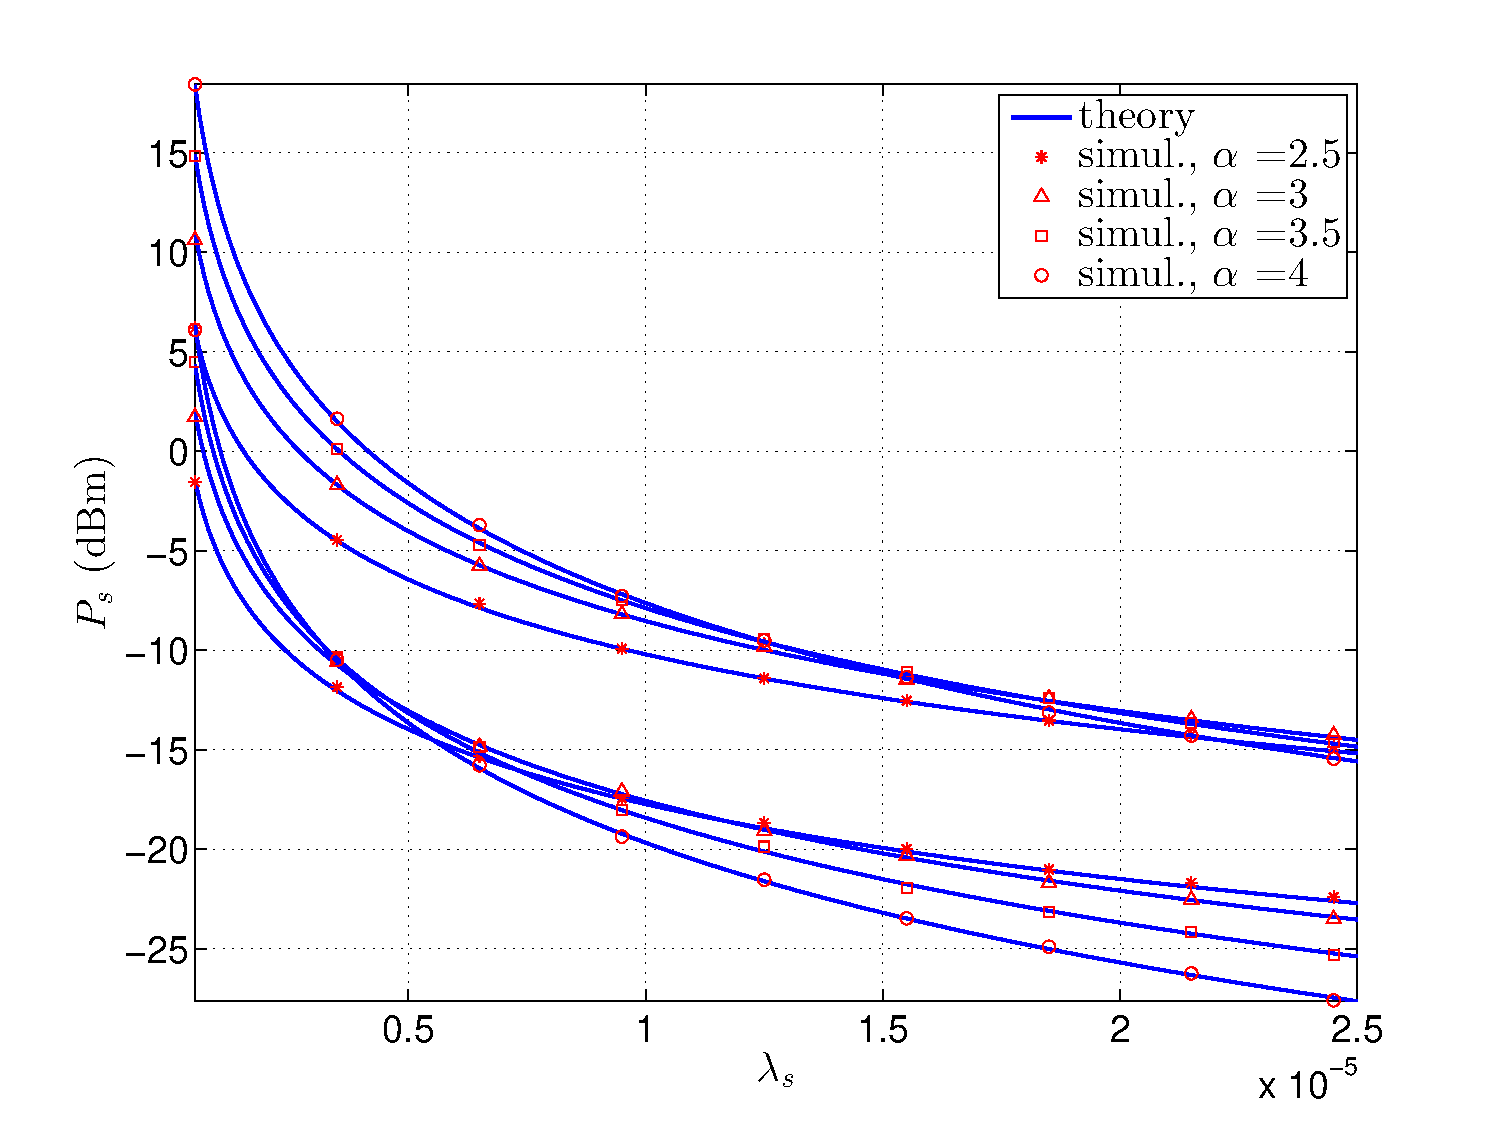
\includegraphics[trim=1.2cm 0.4cm 1.6cm 1.2cm,clip=true,width= 0.42 \paperwidth]{../figures/fig_CR_Txp_vs_lambda_CR_wkr_1e5}
		};
		\begin{scope}[x={(image.south east)},y={(image.north west)}]
			%\draw  (0.832,0.99) node[above=-0.1pt, font=\small] {$I_{\text{th}}$};
			%\draw  (.97,0.898) node[right=-2.2pt, font=\small] {$\epsilon_{\text{I,out}}$};
			%\draw[black,thick,<->] (0.97,0.898) --  node[right=-2.2pt, font=\small] {$\epsilon_{\text{I,out}}$} (0.97,0.985);
			%\draw [thick] (0.831,0.985) -- (0.831,0.096);
			%\draw [thick] (0.08,0.898) -- (0.956,0.898);

			% Select curves depending upon theta   
			\draw (0.65,0.17) arc(-130:130:0.7mm and 3.05mm)  node[above = -0.3mm, font=\tiny] {$d_{\text{p}}$ = 100};
			\draw (0.33,0.47) arc(-130:130:0.7mm and 3.05mm)  node[above= -0.3mm, font=\tiny] {$d\sub{p}$ = 50};
			\draw[black,->] (0.18,0.535) --  node[above = 3.5mm,right, font=\tiny] {$\alpha$} (0.25,0.635);
			\draw[black,->] (0.815,0.22) --  node[above=3.5mm,right, font=\tiny] {$\alpha$} (0.745,0.12);
			
			\draw(0.29,0.715) node[font=\tiny]{Sig. dominant};	
			\draw(0.85,0.305) node[font=\tiny]{Int. dominant};	
		
			%\draw[help lines,xstep=.1,ystep=.1] (0,0) grid (1,1);
			%\foreach \x in {0,1,...,9} { \node [anchor=north] at (\x/10,0) {0.\x}; }
			%\foreach \y in {0,1,...,9} { \node [anchor=east] at (0,\y/10) {0.\y}; }
		\end{scope}
	\end{tikzpicture}
	%\caption{Maximum transmit power of CRs for a given node density $\lambda\sub{s}$, with different choices of $d\sub{p}$ and $\alpha$, where $\theta = 0.95$, $N\sub{p} = \SI{10}{}$, $P\sub{p} = \SI{10}{dBm}$ and $\lambda\sub{p} = 10^{-6} \text{nodes}/{\text{m}^2}$.}
	%\label{fig:tpCR}
	\end{figure}
%	\vspace{-0.5cm}
	\end{overlayarea}
	\vspace{-0.2cm}
	\begin{overlayarea}{\textwidth}{2.2cm}
	\fs{8}
	\begin{table}[t]
        	\renewcommand{\arraystretch}{1.3}
        \centering
        \begin{tabular}{c|c}
        \hline
        	$\theta$  & 0.95 \\ \hline
		$N\sub{p}$ & $\SI{10}{}$ \\ \hline
		$P\sub{p}$ & $\SI{10}{dBm}$ \\ \hline
		$\lambda\sub{p}$ & $10^{-6}\text{nodes}/{\text{m}^2}$  \\ 	
\hline
        \end{tabular}
    \end{table}
    \end{overlayarea}

}
	\end{column}
\end{columns}
%\only<2>
{
	%\footcitetext[(3.29)]{Haenggi08now}
}
%\only<2->
{
	%\vspace{2.0ex}
}
\end{frame}


%%%%%%%%%%%%%%%%%%%%%%%%%%%%%%%%%%%%%%%%%%%%%%%%%%%% Frame %%%%%%%%%%%%%%%%%%%%%%%%%%%%%%%%%%%%%%%%%%%%%%%%%%%%%%	
\begin{frame}[t]{Interference Analysis at ID}
\vspace{-0.2cm}
\begin{columns}
        \begin{column}{0.55\paperwidth}
	%\vspace{-0.06cm}
        \begin{overlayarea}{\textwidth}{7.4cm}
	\begin{itemize}
	\fs{8}
	\item $\mathsf{SIR}\sub{ID}$ at a hypothetical ID
	\begin{align*}
		\mathsf{SIR}\sub{ID} = \frac{P\sub{s}^{*} g\sub{$o$,s} d\sub{s}^{-\alpha}}{\sum\limits_{i \in \Phi_{\text{PT}}} P\sub{p} g_i {\|X_i\|}^{-\alpha} +  \sum\limits_{j \in \Phi_{\text{CR}}} P\sub{s} g_j {\|Y_j\|}^{-\alpha}}. 
	\end{align*}
	\item The outage probability of $\mathsf{SIR}_{\text{ID}}$  
	\begin{align*}
		\mathbb{P}(\textsf{SIR}\sub{ID} < N\sub{s}) = \text{p}\sub{out,s} \equiv \mathbb{P}(\textsf{C}\sub{ID} < R\sub{s}) \\ 
	\end{align*}
	where, $\textsf{C}\sub{ID}$ is capacity at ID, $N\sub{s}$ is $\textsf{SIR}\sub{ID}$ threshold and $R\sub{s}$ is $\textsf{C}\sub{ID}$ threshold at ID.
	\only<2>
	{
		\item Substituting $P\sub{s}^{*}$ from interference analysis at PR 
		\begin{align*}
			p\sub{out,s} = 1 - \left(1 - \epsilon{\sub{p}}\right)^{N\sub{s}^{\frac{2}{\alpha}} m}, \\
\text{where $m = \frac{2 \pi^2 \lambda\sub{s}d\sub{s}^2}{ \alpha \sin\left( \frac{2\pi}{\alpha} \right) \ln \left( \frac{\kappa}{1 - \epsilon\sub{p}} \right) }$}
			\label{eq:SIROutID}
		\end{align*}
	}
	\only<3->
	{
		\item Operating characteristics for the CRN. \\
For given $\psi\sub{s}, \epsilon\sub{p}$ the following must hold 
		\begin{align*}
			\psi\sub{s} \ge \p(\mathsf{C}_{\text{ID}} < R\sub{s}) = 1 - \left(1 - \epsilon{\sub{p}}\right)^{ \left( 2^{R\sub{s}}-1 \right)^{\frac{2}{\alpha}} m }, 
			\label{eq:OC} 
		\end{align*}
	}
	
	\end{itemize}
	\end{overlayarea}
	\end{column}
        
	\begin{column}{0.45\paperwidth}
	\only<4->
	{
	\begin{overlayarea}{\textwidth}{5.1cm}

    %\vspace{-0.6cm}        
	\begin{figure}
		\centering
		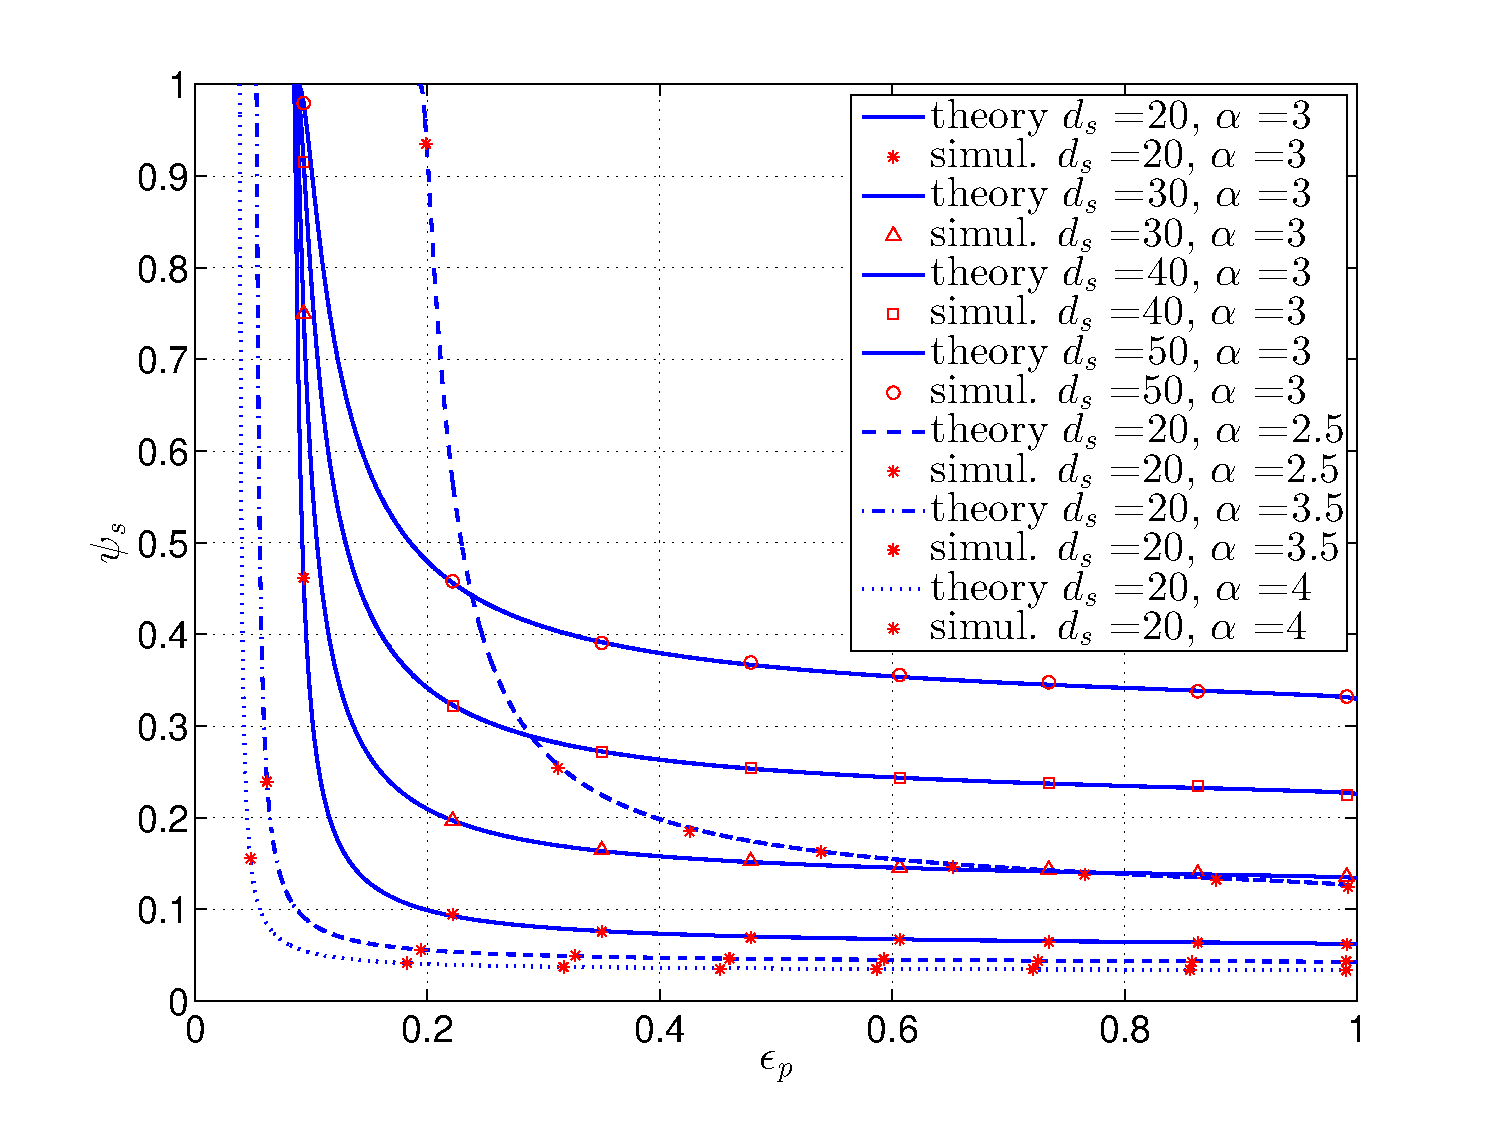
\includegraphics[trim=1.2cm 0.4cm 1.6cm 1.2cm,clip=true,width=0.42 \paperwidth]{../figures/fig_ID_Cap_Out_vs_epsilon_wkr_1e5.pdf}        
	\end{figure}
	\end{overlayarea}
	%\vspace{-0.8cm}
	\begin{overlayarea}{\textwidth}{2.2cm}
	\vspace{-0.9cm}
	\fs{8}
	\begin{table}[t]
        	\renewcommand{\arraystretch}{1.3}
        \centering
        \begin{tabular}{c|c}
        \hline
		$N\sub{p}$ & $\SI{10}{}$ \\ \hline
        	$d\sub{p}$ & $\SI{50}{m}$ \\ \hline
		$P\sub{p}$ & $\SI{10}{dBm}$ \\ \hline
		$R\sub{s}$ & $\SI{2}{bits/sec/Hz}$  \\ \hline 	
		$\lambda\sub{s}$ & $10^{-5}\text{nodes}/{\text{m}^2}$  \\ \hline	
		$\lambda\sub{p}$ & $10^{-6}\text{nodes}/{\text{m}^2}$  \\ 	
\hline
        \end{tabular}
    \end{table}
    \end{overlayarea}

}
	\end{column}
\end{columns}
\end{frame}


%%%%%%%%%%%%%%%%%%%%%%%%%%%%%%%%%%%%%%%%%%%%%%%%%%%% Frame %%%%%%%%%%%%%%%%%%%%%%%%%%%%%%%%%%%%%%%%%%%%%%%%%%%%%%	
\begin{frame}[t]{Performance Analysis at ID}
\vspace{-0.2cm}
\begin{columns}
        \begin{column}{0.55\paperwidth}
        \begin{overlayarea}{\textwidth}{7.4cm}
	\fs{8}
	\begin{itemize}
	\item Consider constraint at PR is fulfilled.
	%Notes:The performance of the secondary system is investigated based on the first and second moments of $\mathsf{C}\sub{ID}$
	\only<2->
	{
		\item The expected capacity at the ID 
		\normalfont
		\begin{align*}
			\e{}{\mathsf{C}_{\text{ID}}} &= \frac{1}{\ln 2} \int\limits_{0}^{\infty} \frac{1}{1+ x} e^{-\mu x^{\frac{2}{\alpha}}} \text{d}x, 
		\end{align*}
		where  $\mu = - m \ln \left({1 - \epsilon{\sub{p}}}\right)$ and $\mu \ge 0$. \newline
		For $\alpha = 4$, 
		\begin{align*} 
			\e{}{\mathsf{C}_{\text{ID}}} &= \frac{1}{\ln 2} \left[ \sin(\mu) \left( \frac{\pi}{2} - \sini(\mu) \right) - \cos(\mu) \cosi(\mu) \right], \label{eq:Exp_Cap_4}  
		\end{align*}
	}
	\only<3->
	{
		\item The variance of capacity at the ID
		\begin{align*}
			\text{Var} [ \mathsf{C}_{\text{ID}} ] &=  \frac{2}{(\ln 2)^2} \int\limits_{0}^{\infty} \frac{\ln(1 + x )}{1 + x} e^{-\mu x^{\frac{2}{\alpha}}} \text{d}x -  {\e{}{\mathsf{C}_{\text{ID}}} }^2. 
			\label{eq:var_cap}
		\end{align*}
	}
	\end{itemize}
	\end{overlayarea}
	\end{column}
        
	\begin{column}{0.45\paperwidth}
	\only<4->
	{
	\begin{overlayarea}{\textwidth}{5.1cm}
	\begin{figure}
		\centering
		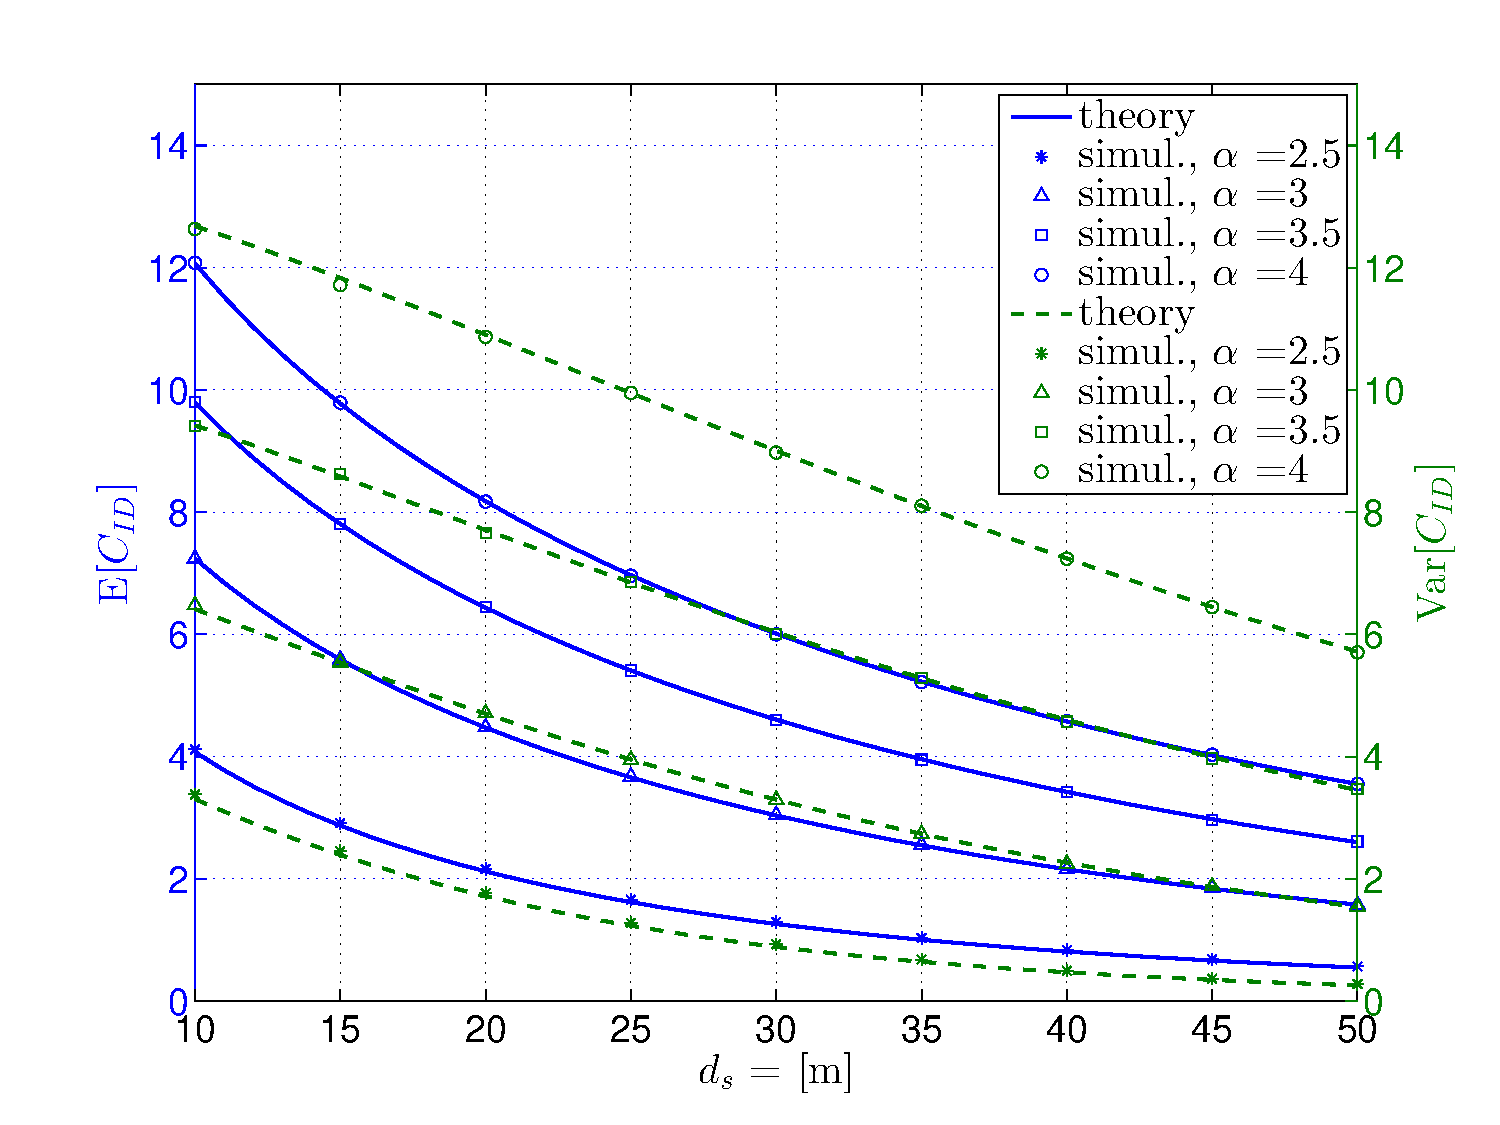
\includegraphics[trim=1.0cm 0.5cm 0.7cm 1.4cm,clip=true,width= 0.42\paperwidth]{../figures/fig_ID_Cap_Moments_vs_d_s_1e5}
	\end{figure}
	\end{overlayarea}
	\begin{overlayarea}{\textwidth}{2.2cm}
	\vspace{-0.8cm}
	\fs{8}
	\begin{table}[t]
        	\renewcommand{\arraystretch}{1.3}
        \centering
        \begin{tabular}{c|c}
        \hline
        	$\theta$  & 0.95 \\ \hline
		$N\sub{p}$ & $\SI{10}{}$ \\ \hline
        	$d\sub{p}$ & $\SI{50}{m}$ \\ \hline
		$P\sub{p}$ & $\SI{10}{dBm}$ \\ \hline
		$\lambda\sub{s}$ & $10^{-5}\text{nodes}/{\text{m}^2}$  \\ \hline	
		$\lambda\sub{p}$ & $10^{-6}\text{nodes}/{\text{m}^2}$  \\ 	
\hline
        \end{tabular}
    \end{table}
    \end{overlayarea}

}
	\end{column}
\end{columns}
\end{frame}


\section{Conclusion}
%%%%%%%%%%%%%%%%%%%%%%%%%%%%%%%%%%%%%%%%%%%%%%%%%%%% Frame %%%%%%%%%%%%%%%%%%%%%%%%%%%%%%%%%%%%%%%%%%%%%%%%%%%%%%	
\begin{frame}{Conclusion}
\fs{8}
\begin{itemize}
\item The paper provides an extension to the concept of cognitive relay to cognitive relay network.
\item Stochastic geometry is used to model the locations of the primary and secondary systems. 
\item  We establish a lower performance bound to benchmark the performance of systems that include model inaccuracies and sensing.
\item Furthermore, we obtain OC to jointly analyze the performance of primary and secondary systems.
\item Based on the expressions obtained and the system parameters defined for an indoor scenario, it is indicated that the CRN operating indoor are propitious for the system. 
\end{itemize}
\end{frame}

\begin{frame}{}
\begin{center}
Thank you for attention! 
\end{center}
\end{frame}

%\printbibliography

\end{document}
